\documentclass[12pt]{article}

% set margins and spacing
\addtolength{\textwidth}{1.3in}
\addtolength{\oddsidemargin}{-.7in} %left margin
\addtolength{\evensidemargin}{-.7in}
\setlength{\textheight}{9in}
\setlength{\topmargin}{-.5in}
\setlength{\headheight}{0.0in}
\setlength{\footskip}{.375in}
\renewcommand{\baselinestretch}{1.0}
\linespread{1.0}

% load miscellaneous packages
\usepackage{csquotes}
\usepackage[american]{babel}
\usepackage[usenames,dvipsnames]{color}
\usepackage{graphicx,amsbsy,amssymb, amsmath, amsthm, MnSymbol,bbding,times, verbatim,bm,pifont,pdfsync,setspace,natbib}
\usepackage{float}

% enable hyperlinks and table of contents
\usepackage[pdftex,
bookmarks=true,
bookmarksnumbered=false,
pdfview=fitH,
bookmarksopen=true,hyperfootnotes=false]{hyperref}

% define environments
\newtheorem{definition}{Definition}
\newtheorem{fact}{Fact}
\newtheorem{result}{Result}
\newtheorem{proposition}{Proposition}



\begin{document}
\title{Shifting Revenue Strategy: The Inverse Relationship Between Consumption Tax and Tariff Revenue in Developed and Developing Countries}
\author{Kathryn Sarrge\thanks{Syracuse University, Economics Students. \newline \indent \indent Email: kesarrge@syr.edu} \and Dylan Thomas \thanks{ dthoma26@syr.edu} \and Umar Bilgrammi \thanks{ujbilgra@syr.edu}}
\date{\vskip-.1in \today}
\maketitle

\vskip.3in
\begin{center} {\bf Abstract} \end{center}

\begin{quote}
{\small We explore the relationship between consumption taxes, such as value added tax (VAT), and tariffs in developed and developing countries to better understand the revenue strategies employed by both groups of countries. Specifically, we explore the correlation between consumption tax and tariffs. We hypothesize that as the share of revenue from consumption taxes increases, the share derived from tariffs decreases, indicating a negative correlation between these two revenue sources.  Using data from the World Integrated Trade Solution (WITS) database, which covers 194 countries from 1988 to 2022, we analyze the two forms of taxation as a percentage of government revenue and consider their implications for economic development. Our findings reveal a moderate negative correlation between consumption tax and tariff revenue in both developing and developed countries, with a correlation coefficient of -0.3255. The implications of this value indicate an inverse relationship between consumption taxes and tariffs in developed and developing countries. Our research synthesizes these findings with the broader literature on tax reform, analyzing why countries opt for tariff revenue or consumption taxes.}
\end{quote}

\bigskip
\section{Introduction} \label{sec:introduction}
The generation of government revenues plays a vital role in shaping the long-term economic stability and growth of a country. According to Michael et al. (1993), in the paper "Integrated Reforms of Tariffs and Consumption Taxes," many countries rely on consumption taxes on goods and services, such as Value Added Tax (VAT), and tariffs on international trade as key sources of revenue. Furthermore, methods to generate revenue vary by country due to various factors including laws, border policies, and a country's economic strengths. Another reading, titled "Tax Challenges Facing Developing Countries," published by Richard M. Bird, Professor Emeritus of the University of Toronto, explores the idea that a country's tax system is always constrained by what it can do. Although both forms of taxation are widely used around the world, our findings suggest an inverse relationship between consumption taxes and tariffs in developing and developed countries. Understanding the relationship between these two forms of taxation-whether they are complements or substitutes-can offer valuable insights for policymakers aiming to optimize tax policies for national development and revenue generation. By analyzing this relationship, we aim to provide critical insights into how governments can maximize their revenue sources. 

This study investigates the relationship between consumption tax and international taxes, such as tariffs, in developed and developing countries. Based on the research question, "Is there an inverse relationship between VAT revenue and tariff revenue in developed and developing countries?", we hypothesize if a consumption tax such as VAT increases in a developed or developing country, then tariffs decrease. Our research question is not designed to investigate whether developed or developing countries have a specific preference towards consumption taxes or international taxes, but rather if there is an inverse correlation that is consistent between both sets of countries. We will examine data from the World Integrated Trade Solution (WITS) database. WITS is an aggregated database that collects economic data from multiple sources and combines it into easily accessible databases for analysis. Our WITS datasets provided information on both forms of taxation as a percentage of government revenue across 194 countries from 1988 to 2022. By analyzing these two key revenue sources, we hope to better understand the fiscal strategies employed by developing and developed nations with an emphasis on if revenue strategies are consistent with each other. 

In this paper, we will present a detailed analysis of the data collected from the WITS database, which includes not only consumption taxes and international taxes but also GDP per capita to help classify countries into developed or developing. We will start with a description of the data, its sources, and variables, followed by a theoretical discussion of the relationship between consumption taxes and international taxes. The results section will outline the correlation between these variables using statistical tests and provide a series of visualizations to illustrate the relationships found within the data. Finally, the paper will conclude with a discussion of the findings, their implications for developing and developed country's fiscal policy, and areas for further research.

\section{Literature Review} \label{sec:literature}

The literature on international and consumption taxes is extensive and highly saturated. Many studies suggest that reducing tariffs while increasing consumption taxes, can improve welfare and maintain or even enhance government revenue. In the paper, "Integrated Reforms of Tariffs and Consumption Taxes" by Michael Et. Al (1993), the idea of reducing tariffs and increasing consumption taxes leads to an improvement in welfare, "Under the conditions specified in Proposition 2 (a mathematical model established in the paper), the integrated reform of the indirect tax structure improves welfare by transferring the function of generating government revenue from high tariff rates to consumption taxes.” Thus, under certain conditions, governments can use a potential inverse correlation to bring positive benefits to their citizens. 

On the other hand, the transfer of tariffs to consumption taxes creates challenges such as partisanship with Government revenue generation.  According to "Taxation and the Political Economy of the Tariff" by John Mark Hansen, "When the government relies fully on a single tax, rates set either too high or too low choke off collections, and both parties are constrained to moderation." If a government were to shift revenues from tariffs to consumption tax, they risk creating an over-reliance on the tax which can result in a loss of profit, failing to deliver increases of welfare to it's citizens. Furthermore, the governments will regress back to moderation in taxes, meaning that if an inverse correlation were to exist between tariffs and consumption taxes it is delicately balanced. In Michael. Et. Al 1993 paper on reforms and welfare, it must be noted that a specific mathematical model and pre-defined conditions resulted in welfare being generated for citizens given the transition from tariffs to consumption tax. 

Similarly, Swarnim Waglé's paper "Coordinating Tax Reforms in the Poorest Countries" published in 2011 poses questions on the transition from trade taxes to domestic consumption taxes. "It is
shown for a sample of low-income countries over 25 years that they have had a mixed record of offsetting reductions in trade tax revenue." This insight is important for understanding the complex and dynamic challenges that developed and developing countries face which hinder the benefits of reducing tariffs in favor of consumption taxes. Thus, the relationship between tariffs and consumption taxes seems to be intricately woven into politics, government structure, and relative income levels. 

Thuy Tien Ho, Xuan Hang Tran, and Quang Khai Nguyen (2023) investigate the link between tax revenue, economic growth, and trade openness, with a focus on developing countries, in their paper, "Tax revenue- economic growth relationship and the role of trade openness in developing countries."  The findings in the paper on the importance of trade openness for economic growth offer a framework in which to contextualize our analysis. Increased trade openness, facilitated by tariff reductions, can potentially support the shift to VAT as a more stable source of revenue, reinforcing the idea that reducing tariffs can have broader positive effects on economic performance, despite the revenue challenges posed to developed and developing countries. 

FIND MORE POSITIVE PAPERS

The general consensus among researchers of the topic is that reducing tariffs and increasing consumption taxes can enhance revenue and welfare, but the success of these reforms depends on a variety of factors. Studies like those of Michael et al. (1993) and Thuy Tien Ho, Xuan Hang Tran, and Quang Khai Nguyen (2023) support the view that such reforms can be beneficial, while Hansen’s (1990) and Swarnim Waglé's 2011 paper juxtapose political economy with tariff reductions, highlighting the difficulties of overcoming tariff policies. All readings acknowledge the potential upsides of reducing tariffs in favor for consumption taxes. Furthermore, the readings analyze a variety of developed and developing countries, allowing for the correlation to be observed as well as it's effects. The highly nuanced and active world of economics creates different challenges for each country, creating volatility which makes it very difficult to conclusively state that reducing tariffs and increasing consumption tax always brings about positive effects for a countries economic development. While most studies support the idea that reducing tariffs and increasing VAT can improve revenue and welfare, they also highlight the importance of political will, effective enforcement, and addressing the informal economy. Our research builds on these findings by specifically examining the inverse relationship between VAT and tariff revenue, contributing to the ongoing discussion of tax reforms in developed and developing countries.

\section{Theoretical Analysis}
\label{sec:theory}
The relationship between consumption taxes and tariffs is diametrically opposed. Tariffs represent taxation of goods which are imported from other countries, while consumption tax represents domestic taxes on production. Thus, the relationship between tariffs and consumption taxes can provide insight to a government's revenue structure. Generally, VAT is considered a more stable and efficient source of revenue than tariffs, especially as countries modernize their taxation as observed in the arguments made by Kowalski, P. 2005, in "Impact of Changes in Tariffs on Developing Countries’ Government Revenue." Tariffs, which are taxes imposed on imports, are often seen as a tool to protect domestic industries, but can be disruptive to trade and economic efficiency. This is because all countries have scarce resources, and thus must rely on other countries exports to make up for their lack of resources in some areas. As countries develop, it is expected that they may shift from relying on tariffs to more consumption-based taxes like VAT for improved revenue generation stability. (Kowalski, P. 2005).

We hypothesize that there is a negative correlation between consumption taxes like VAT and tariff revenue in both developed or developing countries. Since both developed and developing countries are committed to developing further, it is expected that they will continually reduce reliance on tariffs and shift towards encouraging domestic production through increasing consumption taxes. Therefore, our null hypothesis is that increases in consumption taxes do not effect tariffs in developed or developing countries. 

The increase in consumption taxes and decrease in tariffs could reflect a broader trend of globalization, where countries increasingly adopt consumption taxes as part of their fiscal and political strategies, while reducing reliance on trade taxes and making trade easier between borders by lowering associated costs. While it is possible that developed and developing countries may have different preferences for tariffs or consumption tax, it is outside of the scope of this project, which aims to investigate the correlation between taxes and tariffs and see if they are similar in developed and developing countries.

This hypothesis is grounded in the theory of tax modernization, where governments gradually move away from potentially risky taxes like tariffs and towards more efficient taxes like VAT (Kowalski, P. 2005). By examining this relationship, we aim to better landscape of revenue taxation in developing and developed countries.

\section{Data}
\label{sec:data}

We analyzed three time series data sources from the \href{https://wits.worldbank.org/CountryProfile/en/Country/BY-COUNTRY/StartYear/1988/EndYear/2022/Indicator/GC-TAX-GSRV-VA-ZS}{World Integrated Trade Solution} website, which provides detailed information about consumption taxes and tariffs as a percentage of revenue for developing and developed countries. By breaking down tariffs and consumption taxes in terms of percent of revenue, it is easier to observe how much revenue is generated from these taxes, and if they are growing year on year. We utilized a third variable, GDP per capita, which split countries into developed and developing depending on a cutoff value of 12,000 dollars which is derived from the United Nations "World Economic Situation and Prospects 2021" report. The variables in our study are consumption tax, international tax, and GDP per capita. The data entire for the variables span from 1988 to 2022 and cover 194 countries. 

The WITS database aggregates data from various sources. It primarily compiles national statistics on tariffs and taxes from government reports and international organizations. The data collection process involves gathering information directly from the national governments' reports, which are often based on their domestic economic activities, tax laws, and trade statistics. The \href{https://wits.worldbank.org/CountryProfile/en/Country/BY-COUNTRY/StartYear/1988/EndYear/2022/Indicator/GC-TAX-GSRV-VA-ZS}{World Integrated Trade Solution} website provides more information on how they compile their database.

The collection of this data is subject to the availability and reliability of national statistical offices, and differences may arise depending on the country’s data reporting practices. A \href{https://taxsummaries.pwc.com/quick-charts/value-added-tax-vat-rates}{chart} provided by Price-WaterHouse Coopers, a top global consulting firm shows the differences in Value Added Tax rates and reporting across the world. Most notably, Brazil, Ghana, and India report Value Added Tax through three unique approaches. Brazil imposes three levels of value added tax from the federal, state and municipal level, which are between 5-30\%, 17-20\%, and 2-5\%, respectively. Ghana imposes value added tax through a standard rate scheme 15\%, flat rate scheme 3\%, and immovable property 5\%, with additional value added tax on tax applicable supplies. India levies value added tax between 5\% to 28\% depending on the good or service being supplied. Thus, data reporting of Value Added Tax is extremely varied depending on the political structure and a countries interpretation of what counts as value added tax. On the other hand, Tariffs are relatively easy to report due to the Harmonized System developed by the World Customs Organization. Through the Harmonized System, every good is given a code which countries can then use to impose tariffs and disclose them to one another. For example, HS code:0702.00 which through its numbering system refers to tomatoes which are either fresh or chilled. The United States reports its tariffs on goods through the \href{https://hts.usitc.gov/}{Harmonized Tariff Schedule}. The Harmonized Tariff Schedule reveals specific details behind the trading rules, regulations, and methodologies for the United States with regards to certain goods and many countries including but not limited to Singapore, Oman, and Peru to name a few. In conclusion, reporting Value Added Tax is much less standardized than tariffs leading to more entries for tariffs in datasets than value added tax entries, although not by a significant amount.

While the dataset provides information for most countries, certain nations may have incomplete or missing data for specific years. In these cases, either the data is unavailable for that particular year or there are gaps due to inconsistencies in national reporting. For some countries, the data may not start until a later year, and for others, the data may be missing intermittently across the 34-year period. For example, Pakistan has entries for all three variables in consumption tax, international tax, and GDP per capita up until 2001, and then only has entries for GDP per Capita until the end of the dataset. Sri Lanka, a country in South Asia along with Pakistan has entries for all three variables for almost all years. The amount of countries that do not have entries at the start of the period or have no entries during certain periods called holes, is nearly split even. Upon dropping all variables that do not have a value, 2733 observations are left. Of these 2,733 observations, the large majority are developing countries, seemingly showing that the phenomena does differ by development status. This is most likely due to WITS sourcing its some of its data from a database called the UN Comtrade. According to WITS, "The availability of the international trade statistics of UN Comtrade (The United Nations Commodity Trade Statistics database) via the WITS application has been made possible with the permission of the United Nations. UN Comtrade contains annual imports and exports statistics for more than 160 reporting countries or areas, which account for almost all trade worldwide. The trade statistics are detailed giving value and quantity for each commodity broken down by trading partner." Since WITS aggregates various database sources together to create it's databases, some data entries may not encompass all countries, leading to some of the gaps aforementioned above. Furthermore, the UN Comtrade is known to have a significant amount of developing country data, meaning that when WITS aggregates it's databases, it is most likely pulling in more data from developing countries than developed countries. While this does not affect every entry, it may explain why some entries are blank within the data sets. Due to this, we only chose to remove bad data entries from our datasets and left any blank entries as blank, since they would not counted in the statistical tests. 

We acknowledge that the dataset is limited to the data available from the WITS platform, and some countries may have more reliable, consistent reporting than others. For example, it is easy to assume that developed countries often have more accurate and complete records, while developing countries may face challenges in data collection or reporting, but the analysis from WITS has shown the opposite, where developing countries have a more completed record of consumption tax, international tax, and GDP per capita than developed countries did. 

The variables we use in our data are consumption tax, taxes on international trade, and GDP per capita. Consumption tax as a percent of revenue represents the total tax revenue from value added tax or sales taxes divided by total revenue generated. It includes taxes levied on consumption, which can vary greatly across countries as observed in the Price-WaterHouse Coopers chart. Taxes on international trade as a percentage of revenue represents the revenue from tariffs divided by total revenue, providing insight into what proportion tariffs contribute to overall revenue. Finally, GDP per capita represents a country's gross domestic product divided by its population, which is considered an important indicator of the standard of living in a country. In our project specifically, GDP per capita will be used to identify developing and developed countries. Country's that are developed will have a GDP per capita of greater than 12,000 current USD. Countries that are developing with have a GDP per capita that is less than or equal to 12,000 current USD based on the paper "Which Country Is Truly Developed? Covid-19 Has Answered the Ques-
tion" (Freed, Jeffrey S, et al, 2020), and the "World Economic Situation and Prospects 2021" report by the United Nations. For the purpose of our research, countries are evaluated on a year by year basis, therefore a country may be considered developing or developed depending on the year. 

\section{Results}
\label{sec:result}

In this section, we present the analysis of the relationship between taxes on consumption and international tax (tariffs) in developed and developing countries, as described in Section 4. Our primary focus is to investigate the potential inverse relationship between VAT revenue and tariff revenue, and to understand the trends over time. Firstly, we will look at descriptive statistics for all three variables, followed by graphs which provide insight and visualization to the trends and patterns within our data.

The summary statistics for the three variables- taxes on goods and services, taxes on international trade, and gross domestic product—are presented in the table below.  

\begin{table}[h!]
\centering
\caption{Summary Statistics}
\label{tab:summary_stats}
\begin{tabular}{lrrrrr}
\hline
\textbf{Variable} & \textbf{Obs} & \textbf{Mean} & \textbf{Std. Dev.} & \textbf{Min} & \textbf{Max} \\
\hline
gdp              & 6,499        & 11,320.32     & 17,465.2           & 22.85037     & 133,590.1    \\
consumption      & 3,211        & 10.25779      & 5.280867           & 0.0329885    & 40.00499     \\
internatio$\sim$l & 2,969        & 10.24049      & 11.61363           & -0.1304207   & 64.65984     \\
\hline
\end{tabular}
\end{table}


Table 1 provides summary statistics for our three variables. Both international tax and consumption tax are expressed as percentages of total revenue, while GDP is measured in current (2024) U.S. dollars. The mean for both international tax and consumption tax is strikingly similar, at approximately 10.24 percent and 10.26 percent, respectively. However, there are notable differences in their distributions.

The pairwise correlation coefficient test between the international tax and the consumption tax is -.3255. Therefore, these variables have a moderate strength negative correlation. A P-Value of 0.000 is a statistically significant value, meaning that the observed data is highly inconsistent with the null hypothesis giving us reason to reject the null hypothesis. This means there is a statistically significant relationship between tariffs and consumption taxes in developing and developed countries. However, rejection of the null hypothesis does not prove the alternative hypothesis true. Thus, we reject the null hypothesis that there is no relationship between these two variables. 

A significance test done on developing countries reveals a correlation coefficient of -0.3427, with a P-Value of 0.000 giving us further evidence to reject the null hypothesis. A significance test done on developed countries gives a correlation of coefficient of -0.2509, with a P-value of 0.000. Thus, we can confidently reject the null hypothesis and take note that the correlation between consumption tax and tariffs is weaker in developed countries than it is in developing countries. However, it must be noted that this result could be due to the higher amounts of data entries for developing countries. 

A graphical visualization of the whole data is best represented by Figure 1; a scatterplot including international and consumption data. A line of best fit is displayed on the graph, visualizing the negative correlation between international and consumption tax. The data includes information from 194 countries from 1988 to 2022. The x-axis represents consumption tax and y-axis represents international tax, both in terms of percent of revenue. The line of best fit with a negative slope and negative correlation test indicate a moderate inverse relationship between these variables. 

\begin{figure}[h]
    \centering
    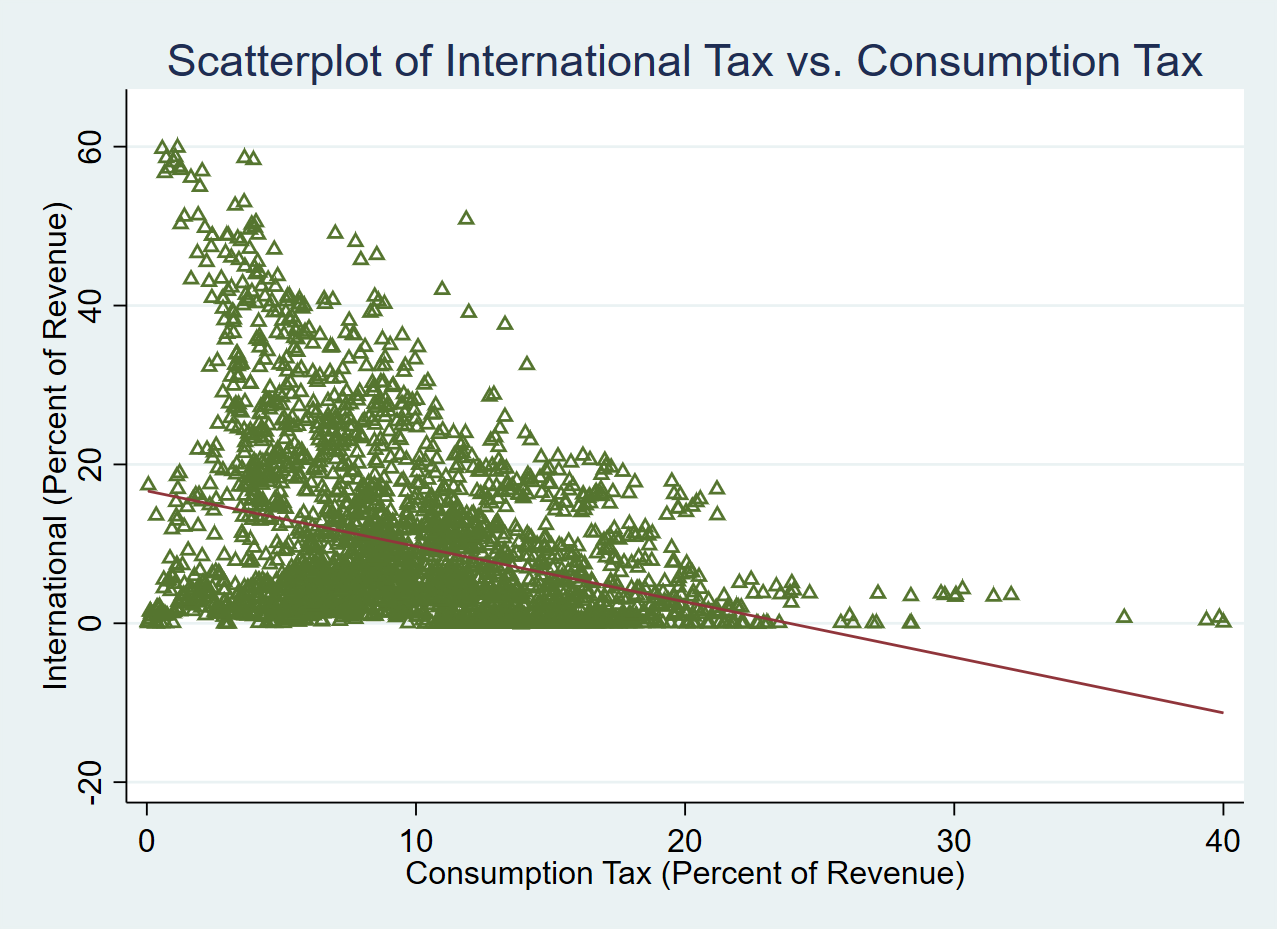
\includegraphics[width=0.5\linewidth]{Reproducibility_Package//research_outputs/Scatterplotintvscons.png}
    \caption{Scatterplot of International tax vs. Consumption Tax}
    \label{fig:enter-label}
\end{figure}

Figure 2 provides a visualization that compares international and consumption tax directly. Consumption tax has a higher density at a lower percent of revenue, while international tax seems to take a larger percent of the revenue than consumption tax at around 10 percent of revenue. 

\begin{figure}[h]
    \centering
    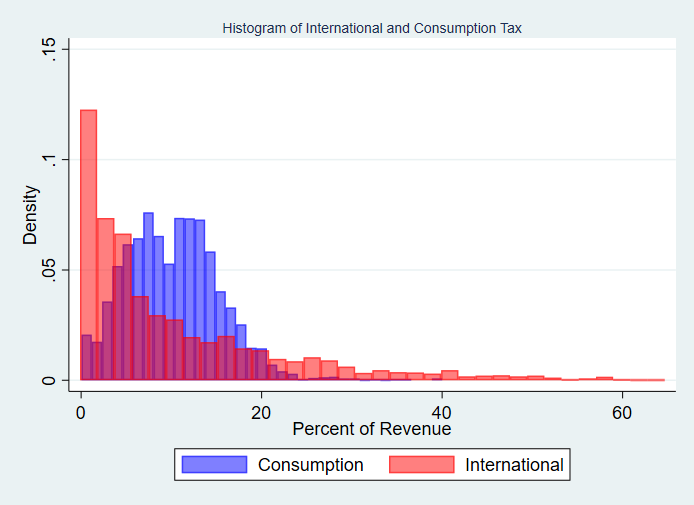
\includegraphics[width=0.5\linewidth]{Reproducibility_Package//research_outputs/twowayhistintcons.png}
    \caption{Histogram of International and Consumption Tax}
    \label{fig:enter-label}
\end{figure}

Figure 3 shows a histogram of international and consumption tax in only developing countries, allowing for comparisons between Figure 2 in how things differ between all countries and just developing countries. In developing countries, consumption tax and international tax seem to much more similar across more revenue percentages in comparison to Figure 2. 

\begin{figure}[h]
    \centering
    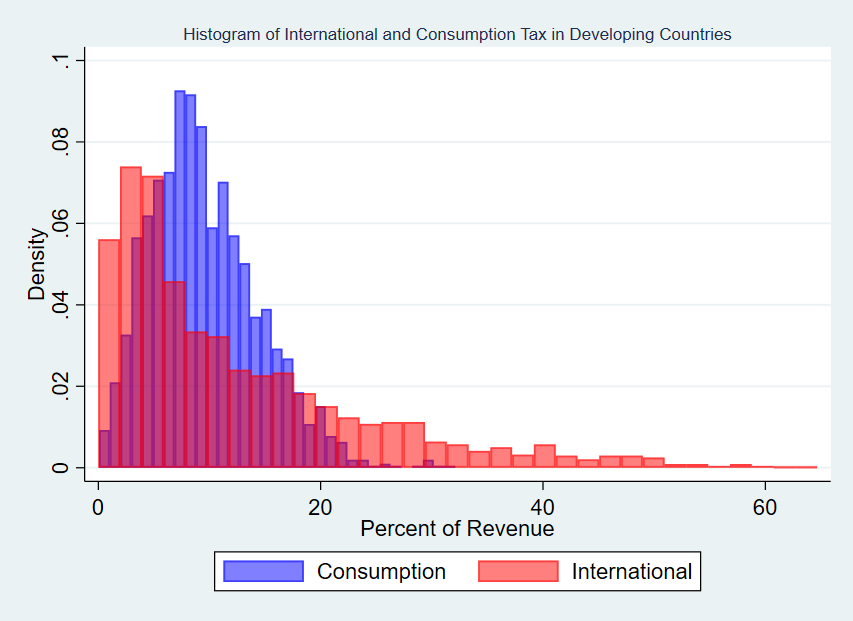
\includegraphics[width=0.5\linewidth]{Reproducibility_Package//research_outputs/twowayhistdevelopingintcons.png}
    \caption{Histogram of International and Consumption Tax in Developing Countries}
    \label{fig:enter-label}
\end{figure}

Figure 4 displays the opposite relationship in comparison to Figure 3. International tax has a higher density in developing countries at lower percentages of revenue in Figure 4, while Figure 3 shows that International has a lower density in developing countries at higher percentages of revenue. 

\begin{figure}[h]
    \centering
    \includegraphics[width=0.5\linewidth]{Reproducibility_Package//research_outputs/twowayhistdevelopedintcons.png}
    \caption{Histogram of International and Consumption Tax in Developed Countries}
    \label{fig:enter-label}
\end{figure}

While the overall trend and correlation indicate a clear relationship between consumption taxes like VAT and tariffs, there are several areas that warrant further investigation. Two particular things that we would like to look further into is specific countries and their relationship between taxes and tariffs and regional differences and how those region have different relationships with taxes and tariffs.

Country-Level Analysis: We could explore time-series graphs for individual countries, particularly those that deviate significantly from the general trend, to identify specific drivers behind these shifts. For example, countries with significant fluctuations in trade policy (e.g., trade liberalization or protectionist measures) could provide insights into how these changes affect the relationship between consumption-based taxes like VAT and tariffs.

Regional Differences: A breakdown of the data by region could shed light on whether the inverse relationship holds across different geographical areas or if regional differences play a role in the strength of this relationship.

In summary, the data suggests a moderate inverse relationship between VAT and tariff revenue in developing countries. This relationship appears to be strengthening over time, reflecting broader shifts in tax systems towards more consumption-based taxation, driven by global economic integration and trade liberalization. However, further exploration at the country and regional levels could provide additional insights into the underlying dynamics.

\section{Conclusion}
\label{sec:conclusion}

In this study, we examined the relationship between consumption taxes and tariff revenue in developing countries, aiming to determine if there is an inverse relationship between these two forms of taxation. By analyzing data from the World Integrated Trade Solution (WITS) database spanning from 1988 to 2022, we found a moderate negative correlation between VAT revenue and tariff revenue across 194 countries. This suggests that, as countries modernize and integrate more into the global economy, they may increasingly rely on consumption-based taxes like VAT while reducing their dependence on tariffs as a source of government revenue.

While our study provides valuable insights into the relationship between consumption tax and tariff revenue in developing countries, several limitations must be acknowledged. One key issue is the quality and completeness of the data. Although the World Integrated Trade Solution (WITS) database is a robust source, the accuracy of data collection can vary across countries, particularly in developing nations where reporting practices may be inconsistent or incomplete. Missing or unreliable data could affect the relevance of our findings and introduce potential biases, especially when analyzing specific countries. 

Overall, this research provides valuable insights for policymakers in developing countries. However, careful attention must be paid to the specific challenges each country faces, particularly in enforcing consumption taxes and addressing the circumstances of their specific economy. Future research should focus on further refining these findings and exploring the political and regional factors that may shape the relationship between consumption taxes and tariffs.



\newpage
\section*{Bibliography}
\singlespacing
\setlength\bibsep{0pt}

Michael, Michael S., Panos Hatzipanayotou, and Stephen M. Miller. "Integrated reforms of tariffs and consumption taxes." Journal of Public Economics 52.3 (1993): 417-428.

Hansen, John Mark. “Taxation and the Political Economy of the Tariff.” International Organization 44.4 (1990): 527–551.

Waglé, Swarnim. "Coordinating tax reforms in the poorest countries: Can lost tariffs be recouped?." World Bank Policy Research Working Paper 5919 (2011).

Ho, Thuy Tien, Xuan Hang Tran, and Quang Khai Nguyen. "Tax revenue-economic growth relationship and the role of trade openness in developing countries." Cogent Business and Management 10(2) (2023)

M. Shahe Emran, Joseph E. Stiglitz, "On selective indirect tax reform in developing countries" Journal of Public Economics 599-623 (2005)

Kowalski, P. (2005), "Impact of Changes in Tariffs on Developing Countries' Government Revenue", OECD Trade Policy Papers, No. 18, OECD Publishing, Paris

Freed, Jeffrey S, et al. “Which Country Is Truly Developed? Covid-19 Has Answered the Question.” Annals of Global Health, U.S. National Library of Medicine, 18 May 2020

Bird, Richard M. (2008), "Tax Challenges Facing Developing Countries" Institute for International Business Working Paper No. 9

Liu Zhenmin, et al. "World Economic Situation and Prospects" United Nations Department of Economic and Social Affairs

United Nations. (2024) "Human Development Insights Database" Human Development Reports Data Center

PriceWater-HouseCoopers. (2024) "Value Added Tax Rates" Worldwide Tax Summaries 

United States International Trade Commission. (2024) "Harmonized Tariff Schedule 2024 HTS Revision 10" United States Government

World Integrated Trade Solutions (2024). "UN Comtrade" Frequently Asked Questions

United Nations (2024). "UN Comtrade Database" United Nations Department of Economic and Social Affairs

Marples, Donald J, "Consumption Taxes: An Overview" Congressional Research Service, January 24, 2023

\newpage
\section*{Data Appendix} \label{sec:appendixa}
\addcontentsline{toc}{section}{Appendix A}

The Data Appendix is used to direct all readers to our \href{https://github.com/ecn310/course-project-taxes-tariffs/blob/main/Reproducibility_Package/README.md}{reproducibility package}. Our reproducibility package contains all of our raw data, modified datasets, do-files to complete statistical analysis, as well as do-files to generate all tables and graphs mentioned in this report. All do-files are commented on each line of code thoroughly explaining the process and methodology in order to get to the final results. 

\end{document}
